\documentclass[../main.tex]{subfiles}
\begin{document}
  \section{Introduction}
    Computer vision is a field concerned with using computers to process and analyze images.
    One of the most important things that human vision is able to do, is object recognition.
    This means that the brain is able to decipher basic information from the eyes, and deduce the objects that can be seen there. %% phrase this better
    This is a complicated task, and not easily replicated programmatically.

    Reliably finding an object within an image is difficult to do at a decent speed.
    Just as there are several ways to describe an object, there are also several different techniques that can be used to locate an object.
    By using as many of these techniques as possible, the reliability of the overall object recognition can be increased.
    Using all available techniques will considerably reduce the speed that objects can be found at.
    This can be mitigated by computing the techniques in parallel, via a task farm.
    This means that general tasks (in this case, each method of identifying an object) will be run concurrently.
    Task farms are especially useful in this case, because it allows the use of libraries that would otherwise be complicated to parallelise.

    A good way of testing the task farm method is with Where's Wally puzzles.
    These are simple cartoons, normally a large image filled with various characters, who wear simply coloured clothing, see Figure \ref{justachump}.
    One of these characters is the eponymous Wally, who is dressed distinctly from the others, see Figure \ref{justwally}.
    Similarly dressed characters exist, Figure \ref{justwenda}, adding complexity to specifically finding Wally.
    The cartoon nature of the characters means that shapes are boldly coloured, and often bordered by a black line.
    As Where's Wally is puzzle, sometimes Wally will be hard to find; he is often obscured, camoflauged or simply small.
    This provides a non-trivial problem, that is still simple enough to provide solutions for.

    \begin{figure}[h]
    \centering
      \begin{subfigure}[b]{0.3\textwidth}
        \centering
        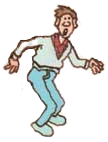
\includegraphics[height=0.15\textheight]{just_a_chump}   
        \caption{A normal person}
        \label{justachump}
      \end{subfigure}
      \begin{subfigure}[b]{0.3\textwidth}
        \centering
        
\includegraphics[height=0.15\textheight]{just_wally}   
        \caption{Wally}
        \label{justwally}
      \end{subfigure}
      \begin{subfigure}[b]{0.3\textwidth}
        \centering
        
\includegraphics[height=0.15\textheight]{just_wenda}   
        \caption{Wenda}
        \label{justwenda}
      \end{subfigure}
    \caption{Characters from Where's Wally}
    \label{wallychars}
    \end{figure}
    \subsection{Shape and Colour Analysis}
    One obvious way of analysing an image with a computer, is to break the image down into shapes and colours.
    In terms of language, it is easiest to depict an object by describing it's shape and colour, i.e. "the red box" or "the green hand".
    This is conceptually simple to explain and understand, and thus is more intuitive to program.
    Most images are saved as raster images (e.g. PNG, BMP, GIF), which is a 2D array of colours that directly map to pixels on a screen.
    This is opposed to vector images that store the location and colour of geometric primitives (squares, circles, triangles, etc.).
    Vector images, rather than raster images, are directly easier to perform shape and colour analysis on.
    However, input devices such as webcams and scanners almost exclusively produce images in raster formats.

    Regardless of format, methods of colour analysis are simple to implement programatically.
    This is because colour is instrinsic to all methods of storing the data of an image.
    Shape analysis is less simple for raster images.
    Shape boundaries must be found, which is normally done through edge detection.
    These boundaries are then analysed to find points of intersection, and the curvature between them.
    The curves, in turn, must then be examined to find what shapes exist.

    These methods allow for a descriptional, heuristic method for locating characters.
    No previous image of Wally is required, only a description, such as "red and white stripes" or "black glasses".
    This allows users to extend the solution past Wally, and towards other characters, who do not have to be seen prior.
    This form of analysis can lead to false positivies, and should be combined with other results.

    An example of the usefulness of this, beyond Where's Wally, could be found in augmented reality technology, such as Google Glass.
    A common problem people experience is losing their keys.
    Users with access to AR devices could use colour and shape analysis to enhance their searching (i.e. if they are visible, but in a cluttered area).
    As keys generally have a few well defined shapes and colour schemes, the device would not have to store what the keys look like in advance.
    Assuming that parallelism is available, this could potentially be done faster than the human eye can search, helping the user significantly.
    
    \subsection{Feature Analysis}
    Some of the most reliable computer vision libraries (such as SIFT \cite{sift}), were developed while considering the neuroscience of human vision.
    Tanaka\cite{tanakahv} and Perrett and Oram\cite{perretthv} found that human object recognition identifies objects with features that are invariant to brightness, scale and position.
    These results have been used as inspiration for feature analysis.
    This finds `feature's, regions of an image which are scale, rotation and illumination invariant.
    These features are most immediately useful when compared with the features of another image.
    For example, the features from an image of just Wally can be used to locate Wally in a normal puzzle image.

    This method generally requires an existing image to find Wally, which leaves 
    However, this method is very reliable, and, as long as Wally is not obscured, will likely locate him.
    Normally, Wally is obscured, so this method should be combined with other techniques.

    Feature analysis benefits from task farming when there is an image needs to be searched for a large number of sub-images.
    A beyond Wally example would be in detecting employees going into work on a flexitime basis.
    This would use photos of each employee combined with CCTV to note the time that workers enter and leave their workplace.
    Users would not need any form of ID other than their own faces, and this can be combined with existing security systems.    
\end{document}
